\newpage
\section{Part 4}
In this section, the implementation of the PID-regulator is done.

We followed the instructions given in the assignment text, and after some documentation reading on the address handling in the Siemens software, we finally got the PID to respond to our set-value. Making new variables required space in memory, hence RECORD taking up 5 bytes from M5.0, we made our variables from M10.0 $\rightarrow$

\begin{figure}[!htb]
    \centering
    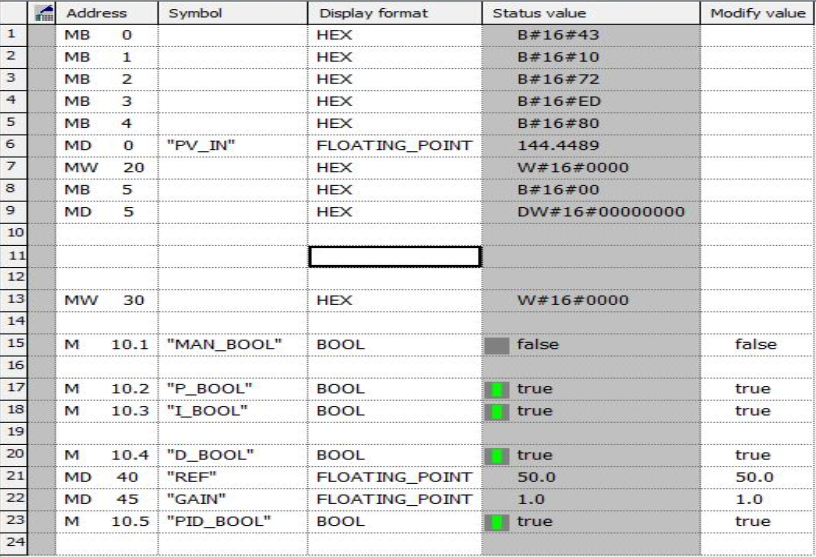
\includegraphics[width=0.8\textwidth]{images/bilde4}
    \caption{VAT\_1}
\end{figure}

\begin{figure}[!htb]
    \centering
    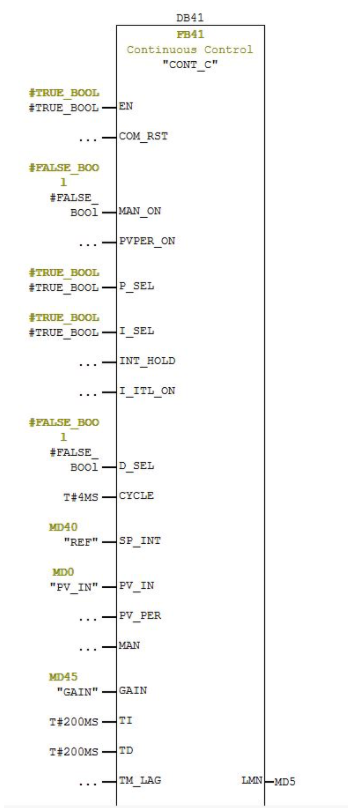
\includegraphics[width=0.6\textwidth]{images/bilde5}
    \caption{PID}
\end{figure}

\begin{figure}[!htb]
    \centering
    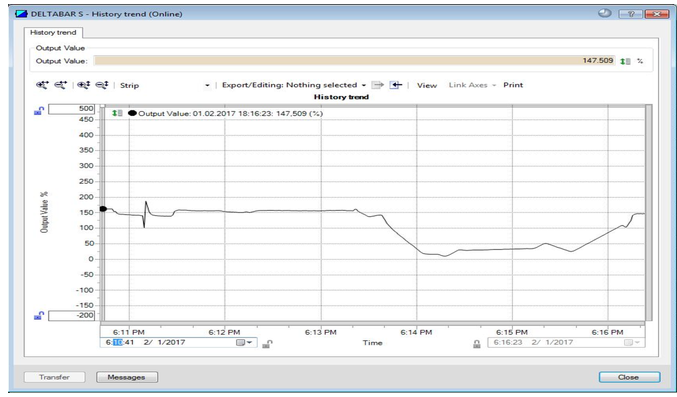
\includegraphics[width=1\textwidth]{images/bilde6}
    \caption{Trend}
\end{figure}

Using PID, requires some values to be found. In a normal situation we would used Ziegler-Nichols methods to find suitable gain, $T_i$ and $T_d$, but due to the valve not working optimal this was rather hard. When the valve exceeded 80$\%$ opening, it got locked. This could maybe be issued by having tightened the seals of the valve too much. Fixing this problem requires mechanical maintenance on the valve, something that one of the lab-responsibles were notified about.

Below, figure 6 is showing a trend over the process, but it is not optimal due to the "locking-valve". To make the valve react after being locked, we needed to send it a 0 signal, release the water pressure and wait approximately 10-15 seconds.


